\documentclass[defaultpackages]{cheatsheet}
\usepackage{kantlipsum, enumitem}

\usepackage{tikzducks}
\usepackage{tikzpeople}

\usepackage{halloweenmath}
\usepackage{coffee4}
\usepackage{slashed}
\usepackage{pgfplots}


\definecolor{fskin}{RGB}{161,140,126}%
\definecolor{fbill}{RGB}{238,212,191}%
\definecolor{fhair}{RGB}{89,72,72}%
\definecolor{crown}{RGB}{255,220,123}
\definecolor{skin}{RGB}{255,215,146}


% This makes the column part of the toc



%\usepackage[-4]{pagesel} % cap at 4 pages+
\pgfplotsset{compat=1.7}

%\usepackage{tikz}
\usetikzlibrary{positioning}
\usetikzlibrary{intersections}
\usetikzlibrary{decorations.pathmorphing}

\ifdefined\isboxes
	\directlua{ require("drawboxes")}
	\usepackage{graphicx,atbegshi}
	\AtBeginShipout {\directlua{drawboxes.visual_debug()}}
 	\usepackage{mathtools}
\fi
\title{Kalkulus 1}
\author{Theodor Tollersrud}
\makeatletter
\newcommand*{\rom}[1]{\expandafter\@slowromancap\romannumeral #1@}
\makeatother
\newcommand*{\myeq}[1]{\stackrel{\mathclap{\normalfont\mbox{$\left(#1\right)$}}}{=}}

\DeclareMathOperator{\rref}{rref}

\newcommand\neginfinf{\stackrel{\mathclap{\normalfont\mbox{$\left[\frac{-\infty}{\infty}\right]$}}}{=}}
\newcommand\infinf{\stackrel{\mathclap{\normalfont\mbox{$\left[\frac{\infty}{\infty}\right]$}}}{=}}
\newcommand\nillnill{\stackrel{\mathclap{\normalfont\mbox{$\left[\frac{0}{0}\right]$}}}{=}}
 
\newcommand*{\skippingparagraph}{\par\vspace{\baselineskip}\noindent}
\newcommand*{\Oe}{\slashed{\mathcal O}}

\usepackage{xparse}

\usepackage{python}

\usepackage{polynom}
 
\polyset{%
   style=C,
   delims={},
   div=:
}

\setdefaultleftmargin{0em}{}{}{}{.5em}{.5em}
\setlength{\plitemsep}{0.5em}

\NewDocumentCommand{\INTERVALINNARDS}{ m m }{
	#1 {,} #2
}
\NewDocumentCommand{\interval}{ s m >{\SplitArgument{1}{,}}m m o }{
	\IfBooleanTF{#1}{
		\left#2 \INTERVALINNARDS #3 \right#4
	}{
		\IfValueTF{#5}{
			#5{#2} \INTERVALINNARDS #3 #5{#4}
		}{
			#2 \INTERVALINNARDS #3 #4
		}
	}
}
\def\doubleunderline#1{\underline{\underline{#1}}}


\renewcommand{\thesubsubsection}{\thesubsection.\alph{subsubsection}}
\setcounter{secnumdepth}{3}
\addtocontents{toc}{\protect\setcounter{tocdepth}{3}}


\pgfmathdeclarefunction{myfunct}{1}{\pgfmathparse{sin(deg(#1)-1.3)+1.72}}


\begin{document}
\begin{center}
	\begin{tikzpicture}
		\duck[santa=red!80!black,
		beard=white!80!brown]
		\end{tikzpicture}
\end{center}
\tableofcontents
	\section{Enkle ting}
\subsection{Polynomdivisjon}
\phantom{}
			$\polylongdiv{x^2-4x+3}{x-3}$
			\rule{\columnwidth}{0.5pt}
			$\polylongdiv[style=D]{x^3-2x^2+4x+7}{x+1}$
			\rule{\columnwidth}{0.5pt}
			$\polylongdiv[style=C]{x^2-2x+4}{x+1}$
	\subsection{Fullføre kvadrat}
	\begin{align*}
		&ax^2+bx+c = a(x+d)^2+e\\
		& d = \frac{b}{2a}\\
		& e = c - \frac{b^2}{4a}
	\end{align*}
	
	\subsection{inf og sup}
	$b$ er en \textit{øvre skranke} til $A$ hvis den er større enn eller lik alle elementene i $A$. Den minste øvre skranke er den \textit{minste øvre skranke} hvis den er den minste av disse. Motsatt er nedre skranke.
	\skippingparagraph
	\textit{minste øvre skranke} $ = \sup A$
	\skippingparagraph
	\textit{største nedre skranke} $ = \inf A$
	\subsection{Begreper}
	\textbf{Konveks}\quad $\cup$\quad $f''(x) > 0$\\
	\textbf{Konkav} \quad $\cap$\quad $f''(x) < 0$
	\subsection{tangent}
	\[y-y_1 = f'(x)(x-x_1)\]
	\subsection{sekant}
	\begin{gather*}
		m = \frac{\Delta y}{\Delta x} = \frac{y_2 - y_1}{x_2 - x_1}\\
		y - y_1 = m(x-x_1)
	\end{gather*}
	\section{Kan være nyttig}
	\subsection{Integral av invers funksjon}
	\phantom{}
	\[\int f^{-1}(y)\,dy = yf^{-1}(y)-F\circ f^{-1}(y) + C\]
	Kan kanskje også løses med og ta arealet av rektangelet fra $a$ til $b$ i $x$-retning og $f(a)$ til $f(b)$ i $y$-retning minus $\int_a^b f(x) \,dx$.
	\subsection{Skrå asymptote}
	\begin{gather*}
		a = \lim_{x\to\infty} \frac{f(x)}{x}\\
		b = \lim_{x\to\infty} f(x) - ax
	\end{gather*}
	Dersom grensene eksisterer, har $f$ en skrå asymptote $ax+b$. Hvis en av grensene ikke finnes, er det ikke noen skrå asymptote.
	\skippingparagraph
	$ax+b$ er en skrå asymptote av $f$ hvis
	\[\lim_{x\to\infty} \left[f(x) - (ax+b)\right] = 0\]
	\subsection{Lengden av en graf}
	Lengden langs en grad fra a til b er gitt ved.
	\begin{gather*}
		L = \int_a^b \sqrt{1+f'(x)}
	\end{gather*}
	\subsection{Numerisk integrasjon}
	Trapesmetoden
	\begin{gather*}
		\int_a^bf(x)\,dx \\
		\approx \frac{\Delta x}{2}\left(f(x_0) + f(x_n) + 2 \sum_{i=1}^{n-1}f(x_i)\right)
	\end{gather*}
	Simpsons metode. Annenhver 2 og 4, unntatt først og sist. 2 på partallsledd, 4 på oddetallsledd.
	\begin{gather*}
		\int_a^bf(x)\,dx \\
		\approx \frac{\Delta x}{3}[f(x_0)+4f(x_1)+2f(x_2)+\cdots\\
		+2f(x_{2n-2}) + 4f(x_{2n-1}) + f(x_{2n})]
	\end{gather*}
	\subsection{Dreie om $x$-aksen}
	Grillspyd
	\begin{gather*}
		V = \int_a^b \pi f(x)^2\,dx
	\end{gather*}
	\subsection{Dreie om $y$-aksen}
	\begin{gather*}
		V = \int_a^b 2\pi xf(x)\,dx
	\end{gather*}
	\section{Komplekse tall}

	$z$ og $w$ er komplekse tall
	\[|z+w|\le |z|+|w|\]
	$z=a+ib$
	\[e^z = e^a(\cos b + i\sin b)\]
	\begin{gather*}
		|z| = \rho = r = \sqrt{a^2+b^2}\\
		a = r\cos\theta\\
		b = r\sin\theta\\
		\cos \theta = \frac{a}{r}\\
		\sin \theta = \frac{b}{r}
	\end{gather*}
	De Moivres formel
	\[(cos \theta + i\sin\theta)^n = \cos(n\theta) + i\sin(n\theta)\]
	\subsection{Trekke røtter av komplekse tall}
	$z=re^{i\theta}$ og $n \in \mathbb{N}$. Da har $z$ nøyaktig $n$ $n$-te røtter, $w_0,\,w_1,\,\cdots,\,w_{n-1}$ som er gitt ved
	\[w_k = r^{1/n}e^{i(\theta + 2k\pi)}\]
	På kartisisk form
	\[r^{1/n} \left(\cos \frac{\theta + 2k\pi}{n} + i \sin \frac{\theta + 2k\pi}{n}\right)\]

	\section{Noen setninger}
	\subsection{Skjæringssetningen}
	Dersom en funksjon har forskjellig fortegn i $a$ og $b$, finnes det et nullpunkt i $[a,\,b]$ hvis funksjonen er kontinuerlig.
	\subsection{Middelverdisetningen}
	Funksjonen $f \,\colon [a, b] \to \mathbb{R}$ er kontinuerlig og deriverbar. Da finnes det et punkt $c$ slik at
	\[f'(c) = \frac{f(b) - f(a)}{b-a}\]
	Enklere forklart så finnes det et punkt $c$ mellom $a$ og $b$ hvis tangent har samme stigningstall som sekanten mellom $a$ og $b$. 
	\resizebox{\columnwidth}{!}{
	\begin{tikzpicture}[declare function={f(\x)=0.3*(\x-3.5)^3-\x+7;a=1;b=6;c=4.94;}]
		\draw[-stealth] (-0.5,0) -- (6.5,0);
		\draw[-stealth] (0,-0.5) -- (0,6.5);
		\draw[blue] plot[smooth,domain=0.5:6.1] ({\x},{f(\x)});
		\foreach \X in {a,b}
		{\draw[dashed] (\X,0) node[below]{$\X$} |- (0,{f(\X)}) node[left] {$f(\X)$};}
		\draw ({a},{f(a)}) -- ({b},{f(b)});
		\draw[dashed] (c,0) -- (c,{f(c)});
		\draw[dashed,name path=hori] (a,{f(a)}) -- (b,{f(a)});
		\pgfmathsetmacro{\slopeangle}{atan2(f(b)-f(a),b-a)}
		\draw[red,name path=sloped] (c,{f(c)})  +(\slopeangle:2) -- ++ (\slopeangle+180:4);
		\draw ({a},{f(a)}) + (1,0) arc(0:\slopeangle:1) node[midway,right]{$\beta$};
		\draw[name intersections={of=hori and sloped,by=i}] (i) +(1,0)
		arc(0:\slopeangle:1) node[midway,right]{$\beta$};
	   \end{tikzpicture}
	}
	\subsection{epsilon-delta}
\hphantom{}
\[\lim_{x\to c} f(x) = L \leftrightarrow (\forall \epsilon,\,\exists\,\delta>0)\]
slik at
\[0 < |x - c| < \delta \Rightarrow |f(x) - L| < \epsilon\]
Gitt en $\epsilon$ så finnes det en $\delta$ slik at om x er så nære c at $|x-c|<\delta$ så er $|f(x) - L|<\epsilon$
\skippingparagraph
$\delta$ er mellom $x$ og $c$; $\epsilon$ er mellom $f(x)$ og $L$.
\[\lim_{h\to 0}\frac{(2+h)^3-2^3}{h} = 12\]
$\epsilon$ er en avstand fra 12. Den er liten som jeg vil. Det som det betyr at grensen eksisterer er at jeg alltid kan finne et interval med input rundt grenseinputtet (0), en avtand $\delta$ unna 0, slik at enhver input innenfor en avtand av $\delta$ gir en output innen avtand $\epsilon$ fra 12, uansett hvor liten $\epsilon$ er (sålenge den er større enn 0). Hvis grensen ikke eksisterer, kan man finne en $\epsilon$ som er for liten, til å finne en $\delta$
\resizebox{\columnwidth}{!}{
\begin{tikzpicture}[
	>=stealth, %% arrow tips
]
\begin{axis}[
		blue,
		axis x line=middle,
		axis y line=center,
		every axis x label/.style={at={(current axis.right of origin)},anchor=north},
		every axis y label/.style={at={(current axis.above origin)},anchor=east},
		xmin=-0.5,xmax=1.5,
		ymin=-0.5,ymax=3,
		xtick=\empty,
		ytick=\empty,
		xlabel={$x$},
		ylabel={$y$},
	]

	%% draw the plot:
	\addplot [red,samples=100] {myfunct(x)};

	%% define some coordinates that we need later:
	\def\xa{0.25}
	\pgfmathsetmacro{\ya}{myfunct(\xa)}
	\path (axis cs:\xa, \ya) coordinate (0);

	\def\xb{0.5}
	\pgfmathsetmacro{\yb}{myfunct(\xb)}
	\path (axis cs:\xb, \yb) coordinate (1);

	\def\xc{0.75}
	\pgfmathsetmacro{\yc}{myfunct(\xc)}
	\path (axis cs:\xc, \yc) coordinate (2);

	\path (axis cs:0, 0) coordinate (origin);
\end{axis}

%% draw the black lines:
\tikzset{marker/.style={shorten <=-3pt,shorten >=-3pt}} %% expand the lines
\draw [marker] (origin-|0) -- (0);
\draw [marker] (origin|-0) -- (0);
\draw [marker] (origin-|1) -- (1);
\draw [marker] (origin|-1) -- (1);
\draw [marker] (origin-|2) -- (2);
\draw [marker] (origin|-2) -- (2);

%% δ, ε:
\path (origin) ++(10pt,10pt) coordinate (offset);

\draw [<->,red!50!blue] (offset-|0) -- node [above] {$\delta$} (offset-|1);
\draw [<->,red!50!blue] (offset-|1) -- node [above] {$\delta$} (offset-|2);
\node at (origin-|1) [below,yshift=-3pt,red!50!blue] {$c$};

\draw [<->,black!50!blue] (offset|-0) -- node [right] {$\varepsilon$} (offset|-1);
\draw [<->,black!50!blue] (offset|-1) -- node [right] {$\varepsilon$} (offset|-2);
\node at (origin|-1) [left,xshift=-3pt,black!50!blue] {$L$};
\end{tikzpicture}
}
	\section{Differensligninger}
	Formen $x_{n+2} + bx_{n+1}+cx_n=0$. Løs den karakteristiske ligningen $r^2+bx + c = 0$.
	\subsection{To reelle røtter}
	\begin{gather*}
		x_{n} = Cr_1^n+Dr_2^n
	\end{gather*}
	\subsection{\'En reell rot}
		\begin{gather*}
			x_n = Cr_1^n+Dnr_1^n
		\end{gather*}
	\subsection{Komplekse røtter}
	\begin{gather*}
		x_{n+2} + bx_{n+1}+cx_n=0\\
		x_n = Cr^n+\overline{C}\overline{r}^n\tag{reelle løsninger}\\
		x_n = E\rho^n\cos(n\theta)+F\rho^n\sin(n\theta)\tag{trigonmetrisk form for reelle løsninger}
	\end{gather*}
	\subsection{Inhomogene}
	Fungerer på samme måte og har samme fremgangsmåte som inhomogene differensialligninger.
	\section{Integrering}

	\subsection{Delvis integrasjon}
	\phantom{}
	\[\int F\cdot g \;dx = F\cdot G-\int f\cdot G\;dx\]
	\subsection{Substutisjon}
	\phantom{}
	\begin{align*}
		&\int f(g(x))g^\prime(x)dx\\
		& u = g(x)\\
		& \frac{du}{dx} = g^\prime(x)\\
		& dx = \frac{du}{g^\prime(x)}\\
		& \int f(u)g^\prime(x) \frac{du}{g^\prime(x)}\\
		& \int f(u)\,du
	\end{align*}
	\subsection{Delbrøkoppspaltning}
	P og Q er polynomer
	$$\int \frac{P(x)}{Q(x)}\;dx$$

	\begin{compactenum}
		\item $\deg(P) \ge \deg(Q) \Rightarrow$ utfør polynomdivisjon
		\item Faktoriser $Q$ i reelle første- og annengradsuttrykk. Sjekk at annengradsuttrykkene ikke kan faktoriseres ytterligere.
		\item Foreta delbrøkoppspaltning. Integralene vi nå har er på formen $\int \frac{A}{(x-r)^n}\;dx$ eller $\int \frac{Bx+C}{(x^2+ax+b)^m}\;dx$. Den første typen kan integreres umiddelbart.
		\item For å integrere den andre typen, smugler du den deriverte til $x^2+ax+b$ inn i $P$, og substituerer $u=x^2+ax+b$. Du står igjen med et integral på formen $\int \frac{dx}{(x^2+ax+b)^m}$.
		\item Fullfør kvadratet og substituer slik at integralet får formen $\int \frac{du}{(1+u^2)^m}$.
		\item Bruk rekursjonsformelen til å redusere multiplisiteten m. Til slutt sitter du igjen med $\int \frac{du}{1+u^2}$ som kan integreres direkte.
	\end{compactenum}
	Rekursjonsformelen
	\begin{align*}
	I_m =& \int\frac{du}{(1+u^2)^m}\\
	I_m =& \frac{1}{2(m-1)}\cdot\frac{u}{(1+u^2)^{m-1}}\\
	+& \frac{2m-3}{2(m-1)}I_{m-1}
	\end{align*}
	\subsubsection{Eksempler}
	\paragraph{Kan ikke faktoriseres, men smuglingen er veldig lett}
	\begin{align*}
		I &= \int \frac{x+2}{x^2+4x+6}\;dx\\
		P(x) &= x+2\\
		Q(x) &= x^2+4x+6\\
		&\text{Q kan ikke faktoriseres}\tag{2}\\
		&\text{Vi har form 2}\tag{3}\\
		\frac{d}{dx}Q(x) &= 2x + 4\\
		&\text{Vi smugler $Q'$ inn i $P$}\tag{4}\\
		I &= \frac{1}{2}\int \frac{2x+4}{x^2+4x+6}\; dx\\
		u&=x^2+4x+6\\
		dx &= \frac{du}{2x+4}\\
		I &= \frac{1}{2} \int \frac{1}{u}\;du\\
		I&= \frac{1}{2}\ln|u|+C\\
		I&= \doubleunderline{\frac{1}{2}\ln|x^2+4x+6|+C}
	\end{align*}
	\paragraph{Kan faktoriseres}
	\phantom{}
	\begin{align*}
		&I = \int \frac{2x+1}{x^2-4x+3}\;dx\\
		&x^2 - 4x + 3 = (x-1)(x-3)\\
		& \frac{2x+1}{(x-1)(x-3)} = \frac{A}{x-1}+\frac{B}{x-3}\\
		&\text{gange med felles nevner $(x-1)(x-3)$}\\
		&2x + 1 = A(x-3) + B(x-1)\\
		&x = 1 \Rightarrow 2\!\cdot\!1\!+\!1 = A(1\!-\!3) + B(1\!-\!1)\\
		& 3 = -2A\\
		& A = \frac{-3}{2}\\
		& x = 3 \Rightarrow 2 \cdot 3 + 1 = A\cdot 0 + B(3-1)\\
		& 7 = 2B\\
		& B = \frac{7}{2}\\
		& \frac{2x+1}{x^2-4x+3} = \frac{-\frac{3}{2}}{x-1} + \frac{\frac{7}{2}}{x-3}\\
		& I = -\frac{3}{2}\int \frac{1}{x-1}\;dx + \frac{7}{2}\int \frac{1}{x-3}\;dx\\
		& I = \doubleunderline{-\frac{3}{2} \ln |x-1| + \frac{7}{2}\ln|x-3|+C}
	\end{align*}
	\paragraph{En jævel}
	\begin{align*}
		& I = \int \frac{x+1}{(x-1)(x^2+x+1)}\;dx\\
		& \frac{x+1}{(x\!-\!1)(x^2\!+\!x\!+\!1)}\!=\!\frac{A}{x\!-\!1}+\frac{Bx+C}{x^2\!+\!x\!+\!1}\\
		& \text{Ganger med $(x-1)(x^2+x+1)$}\\
		& (x\!+\!1)\!=\!A(x^2\!+\!x\!+\!1)\!+\!(Bx+C)(x\!-\!1)\\
		&=Ax^2\!+\!Ax\!+\!A\!+\!Bx^2\!-\!Bx\!+\!Cx\!-\!C\\
		&=x^2(A\!+\!B)+x(A\!-\!B\!+\!C)+(\!A-\!C)
	\end{align*}
	For at dette skal være lik $x+1$, får vi ligningssystemet
	\begin{align*}
		A+B &= 0 \\ 
		A-B+C &= 1 \\ 
		A-C &= 1
	  \end{align*}
	  Vi løser selvsagt dette med
	  \[
		  \rref\left(
	  \begin{bmatrix}
		  1&1&0&0\\
		  1&-1&1&1\\
		  1&0&-1&1
	  \end{bmatrix}
		  \right) \]
		  \vspace{1em}
		  \[= \begin{bmatrix}
			  1&0&0&\frac{2}{3}\\
			  0&1&0&-\frac{2}{3}\\
			  0&0&1&-\frac{1}{3}
		  \end{bmatrix}
	  \]
	  Vi har således\[
		  A=\frac{2}{3}\quad  B=-\frac{2}{3}\quad C=-\frac{1}{3}
	  \]
		  \begin{align*}
			  &I=\int\frac{\frac{2}{3}}{x-1}+\frac{-\frac{2}{3}x-\frac{1}{3}}{x^2+x+1}\;dx\\
			  &\text{Vi ganger med $-\frac{1}{3}$ for at}\\
			  &\text{telleren er lik nevneren derivert}\\
			  &= \frac{2}{3}\ln|x-1|-\frac{1}{3}\int \frac{2x+1}{x^2\!+\!x\!+\!1}dx\!+\!C\\
			  & u = x^2+x+1\tag{teller er lik $\frac{du}{dx}$!}\\
			  & \frac{du}{dx} = 2x+1\\
			  & dx = \frac{1}{2x+1}du\\
			  &I = \frac{2}{3}\ln |x-1|\!-\!\frac{1}{3}\int \frac{2x\!+\!1}{u}\cdot\frac{1}{2x\!+\!1}du\\
			  &I = \frac{2}{3}\ln|x-1|-\frac{1}{3}\int \frac{1}{u}\;du+C\\
			  &I = \doubleunderline{\frac{2}{3} \ln |x-1| -\frac{1}{3}\ln|x^2+x+1|+C}
		  \end{align*}
	\subsection{Definisjon}
	partisjon av intervallet $[a,\,b]$ er en endelig mengde $\Pi = \{x_0,\,x_1,\,\cdots,\,x_n\}$ slik at 
	\[a = x_0<x_1<\cdots<x_n=b\]
	\begin{align*}
		&M_i = \sup\{f(x) \,\colon x\in [x_{i-1},\,x_i]\}\tag{$\max(f(x_i), f(x_{x-1}))$}\\
		&m_i = \inf\{f(x) \,\colon x\in [x_{i-1},\,x_i]\}\tag{$\min(f(x_i), f(x_{x-1}))$}\\
		&\Oe(\Pi) = \sum_{i=1}^{n} M_i(x_i-x_{i-1})\\
		&\mathcal{N}(\Pi) = \sum_{i=1}^n m_i(x_i-x_{i-1})\\
		&\overline{\int_a^b} f(x) dx = \inf\{\Oe(\Pi)\,\colon\text{alle mulige } \Pi\}\\
		&\underline{\int_a^b} f(x) dx = \inf\{\mathcal{N}(\Pi)\,\colon\text{alle mulige } \Pi\}
	\end{align*}
	Dersom $\overline{\int_a^b} f(x) dx = \underline{\int_a^b} f(x) dx$ er $f$ integrerbar
	\subsection{Tips}
	\subsubsection{$\int \sqrt[n]{\frac{ax+b}{cx+d}}$}
	Substituer $u=\sqrt[n]{\frac{ax+b}{cx+d}}$\\
	Løs for $x$, deriver, finn $\frac{dx}{du}$ og deretter $dx$
	\[I = \int u \,dx\]
	Dette kan løses med delbrøkoppspaltning
	\subsubsection{$\int R(\sin x, \cos x)$}
	\begin{gather*}
		R(\sin x, \cos x)=\\
		 \frac{\displaystyle\sum_{n=0}^N\sum_{m=0}^M a_{n,m}\sin^n x\cos^m x}{\displaystyle\sum_{n=0}^L\sum_{m=0}^K b_{n,m}\sin^n x\cos^m x}
	\end{gather*}
	Substituer $u=\tan\frac{x}{2}$
	\begin{gather*}
		\sin x = \frac{2u}{1+u^2}\\
		\cos x = \frac{1-u^2}{1+u^2}\\
		dx = \frac{2}{1+u^2}\,du
	\end{gather*}
\section{Newtons metode}
	\phantom{}
	\[x_{n+1} = x_n - \frac{f(x_n)}{f^\prime(x_n)}\]
	Anta at $f(a)=0$, at $f^\prime(a)\neq 0$ og at $f^{\prime\prime}(x)$ eksisterer og er kontinuerlig rundt $a$. Da finnes det en $\delta > 0$ slik at følgen $\{x_n\}$ i Newtons metode konvergerer mot $a$ når $x_0\in (a-\delta,\,a+\delta)$. 
	\section{Diffligninger}
	\subsection{Førsteordens lineære}
	\begin{align*}
		&y^\prime + f(x)y = g(x)\\
		&y = e^{-F(x)}\left(\int e^{F(x)}g(x)\,dx + C\right)
	\end{align*}
\subsection{Annenordens homogen med konstante koeffisienter}
\begin{align*}
	&y^{\prime\prime}+py^\prime+qy=0\\
\end{align*}
	$y_1$ og $y_2$ er løsninger. Da er også
	$$y = Cy_1 + Dy_2$$
	en løsning med alle $C$ og $D$.
	For å finne $y_1$ og $y_2$ løser vi den karakteristiske ligningen
	\[r^2+pr + q = 0\]
	\paragraph{To røtter}
	Dersom vi har to røtter er
	\[y = Ce^{r_1x} + De^{r_2x}\]
	Vi vet at $r_1+r_2=-p$
	\paragraph{\'En rot}
	\[y=Ce^{r_1x}+Dxe^{r_1x}\]
	\paragraph{Komplekse røtter}
	To røtter $r_1=a+ib$ og $r_2 = a-ib$
	\[y=e^{ax}(C\cos(bx)+D\sin (bx))\]

\subsection{Annenordens inhomogen}
\begin{align*}
	y^{\prime\prime} + py^\prime + qy = f(x)
\end{align*}
Vi tipper $y_p(x)$ er på formen:
Dersom f(x) er et polynom sier vi at g(x) er et polynom av samme grad som f, og forsøker

gitt multisettet $\Omega$ er løsningene til den karakteristiske ligningen $r^2 + pr + q = 0$
\begin{tabular}{|c|c|}
	\hline
	er 0 en rot?& $y_p$\\\hline
	$0 \notin \Omega$ & $g(x)$\\
	$0 \in^1 \Omega$ & $xg(x)$\\
	$0 \in^2 \Omega$ & $x^2g(x)$\\
	\hline
\end{tabular}

Gitt funksjonen $\Upsilon\; \colon M \times \mathbb{R} \to \mathbb{N}$, gir multiplisiteten til et tall i et multiset, har vi
\[y_p = x^{\Upsilon(\Omega, 0)}g(x)\]

Dersom vi har formen $f(x) = e^{ax}P(x)$ der P er et polynom, tipper vi
\[y_p = e^{ax}x^{\Upsilon(\Omega, a)}Q(x)\]
der $Q$ er et polynom av samme grad som $P$.

Dersom vi har formen $$f(x) = a^x(A\cos (bx) + B\sin (bx))$$ tipper vi
\[y_p = a^x(C\cos(bx) + D\sin(bx))\]

Dersom $a^x\cos(bx)$ eller $a^x\sin(bx)$ er den karakteristiske ligningen tipper vi
\[y_p = x\cdot a^x(C\cos (bx) + D\sin (bx))\]


\subsubsection{Fremgangsmåte for å løse}
\begin{compactitem}
	\item Løs $r^2 + pr + q = 0$
	\item Finn $y_h = Ce^{r_1x}+De^{r_2x}$
	\item Med komplekse røtter blir det annerledes, se over.
	\item Ukjente koeffisienters metode
	\item Gjett $y_p$ og finn $y_p^\prime$ og $y_p^{\prime\prime}$
	\item Innsett i ligningen
	\item Løs ligningsstystemet og finn $A$ og $B$
	\item Vi har funnet den partikulære løsningen.
	\item Den generelle er $y=y_p+y_h$
	\item Dersom du har $y(0)=\alpha$ og $y^\prime (0) = \beta$, løs ligningssystemet og finn $C$ og $D$.
\end{compactitem}
\subsubsection{Parametervariasjon}
\textbf{Last minute resort}
\begin{align*}
	&y^{\prime\prime} + py^\prime + qy = f(x)\\
	& y = Cy_1 + Dy_2  \tag{$y_n = e^{r_nx}$}\\
	& \text{Vi erstatter $C$ og $D$ med $c(x)$ og $d(x)$}\\
	& y = c(x)y_1(x)+d(x)y_2(x)\\
	& c(x) = - \int \frac{y_2(x)f(x)}{W(y_1,y_2)} dx\\
	& d(x) = \int \frac{y_1(x)f(x)}{W(y_1,y_2)} dx\\
	& W(y_1, y_2) = y_1y_2^\prime - y_1^\prime y_2
\end{align*}

Dette er den generelle løsningen, ikke den homogene! M.a.o. så er man ferdig!

\subsection{Separable Diffligninger}
Kan skrives på formen
\[q(y)y^\prime = p(x)\]
For å løse
\[\int q(y)y^\prime \, dx = \int p(x)\,dx\]
$dy=y^\prime\,dx$ ergo.
\[\int q(y) dy = \int p(x)\,dx\]'
Regn integralene og løs mhp. $y$.
	\section{Taylorpolynom}
Taylorpolynomet til $f$ av grad $n$ om punktet $a$ er gitt ved
\[T_nf(x;\,a) = \sum_{k=0}^n\frac{f^{(k)}(a)}{k!}(x-a)^k\]
(der $f^{(k)}(a) = \frac{d^kf}{dx^k} (a)$ og $f^{(0)}(a)=f(a)$)


\addtocontents{toc}{\protect\setcounter{tocdepth}{1}}
	\section{Hjemmeeksamen}
	\begin{tikzpicture}
		\duck[graduate=gray!20!black,
		tassel=red!70!black]
		\end{tikzpicture}
	\subsection{}
	\subsubsection{}
	\begin{align*}
		z^2+\sqrt{3}z+1&=0\\
		z&=\frac{-\sqrt{3} \pm \sqrt{(\sqrt{3})^2 - 4}}{2}\\
		z&=\frac{-\sqrt{3} \pm -\sqrt{-1}}{2}\\
		z = \frac{-\sqrt{3}}{2} + \frac{1}{2}i &\vee z = \frac{-\sqrt{3}}{2} - \frac{1}{2} i\\
		z_1 = \rho e ^ {i\theta_1}\quad&\quad z_2 = \rho e ^ {i\theta_2}\\
	\end{align*}
	\begin{align*}
		\rho &= \sqrt{(\Re z)^2 + (\Im z)^2}\\\
		\rho &= \sqrt{\left(-\frac{\sqrt{3}}{2}\right)^2\!\!+\!\left(\frac{1}{2}\right)^2}\\
		\rho &= \sqrt{\frac{3}{4} + \frac{1}{4}} = 1\\
		\cos \theta = \frac{\Re z}{\rho} \quad & \quad \sin \theta = \frac{\Im z}{\rho}\\
		\cos \theta_1 &= \frac{-\frac{\sqrt{3}}{2}}{1} = -\frac{\sqrt{3}}{2}\\
		\sin \theta_1 &= \frac{\frac{1}{2}}{1} = \frac{1}{2}\\
	\end{align*}
	\(z_1\) er i \rom{2} kvadrant
	\begin{align*}
		\theta_1 = \frac{5}{6}\pi\\
		\cos \theta_2 &= \frac{-\frac{\sqrt{3}}{2}}{1} = -\frac{\sqrt{3}}{2}\\
		\sin \theta_2 &= \frac{-\frac{1}{2}}{1} = -\frac{1}{2}\\
		z_2 \text{ er i \rom{3}}&\text{ kvadrant}\\
		\theta_2 = \frac{7}{6}\pi\\
		z_1 = e^{i\frac{5}{6}\pi}\quad&\quad z_2=e^{i\frac{7}{6}\pi}\\
	\end{align*}
		\subsubsection{}
	$f(x) = x$ er et polynom av første grad. Vi bruker ukjente koefisienters metode. Løsningen er kanskje på formen $Ax+B$
	\begin{align*}
		y_p &= Ax + B\\
		y^{\prime\prime}_p + \sqrt{3}y_p^\prime + y_p &= 0 + \sqrt{3}A + B\\
		x=0&\Rightarrow\sqrt{3}A + B = 0\\
		x=1&\Rightarrow A\!+\!\sqrt{3}A\!+\!B=1\\
		B&=-\sqrt{3}A\\
		A + \sqrt{3}A - \sqrt{3}A &= 1\\
		A &= 1\\
		\sqrt{3} + B &= 0\\
		B &= -\sqrt{3}\\
		y_p = x - \sqrt{3} \quad&\text{Partikulær løsning}
	\end{align*}
	Vi finner $y_h$
	\begin{align*}
		&r^2 + \sqrt{3}r + 1 = 0\\
		&r = -\frac{\sqrt{3}}{2} + \frac{1}{2}i \vee r = -\frac{\sqrt{3}}{2} - \frac{1}{2}i\\
		&y_h = Ce^{\left(-\frac{\sqrt{3}}{2} + \frac{1}{2}i\right)x}+  De^{\left(-\frac{\sqrt{3}}{2} - \frac{1}{2}i\right)x}\\
		&= Ce^{-\frac{\sqrt{3}}{2}x + \frac{1}{2}ix} + De^{-\frac{\sqrt{3}}{2}x - \frac{1}{2}ix}\\
		&= Ce^{-\frac{\sqrt{3}}{2}x} \cdot e^{\frac{1}{2}ix} + De^{-\frac{\sqrt{3}}{2}x} \cdot e ^ {-\frac{1}{2}ix}\\
		&= Ce^{-\frac{\sqrt{3}}{2}x} \cdot \left(\cos\frac{x}{2} + i\sin{\frac{x}{2}}\right)\\
		&+De^{-\frac{\sqrt{3}}{2}x} \cdot \left(\cos\frac{-x}{2} + i\sin\frac{-x}{2}\right)\\
		&= Ce^{-\frac{\sqrt{3}}{2}x} \cdot \left(\cos\frac{x}{2} + i\sin{\frac{x}{2}}\right)\\
		&+De^{-\frac{\sqrt{3}}{2}x} \cdot \left(\cos\frac{x}{2} - i\sin\frac{x}{2}\right)\\
		&y = y_p + y_h\\
		&y = x - \sqrt{3} + y_h
	\end{align*}
	\subsection{}
	\subsubsection{}
	\begin{align*}
		&\lim_{x\to 0} \frac{\arcsin x - \sin x}{x^2}\\
		\myeq{\frac{0}{0}}&\lim_{x\to 0} \frac{\frac{1}{\sqrt{1-x^2}} - \cos x}{2x}\\
		\myeq{\frac{0}{0}}&\lim_{x\to 0} \frac{x(1-x^2)^{-\frac{3}{2}}+\sin x}{2} = 0
	\end{align*}
	\subsubsection{}
	\begin{align*}
	&\int \frac{\arctan x \ln \arctan x}{1+x^2} \;dx\\
	u &= \arctan u\\
	\frac{du}{dx}&= \frac{1}{x^2+1}\\
	dx &= (x^2+1)\;du\\
	&\int u \ln u \; du\\
	=& \frac{1}{2} u^2 \ln u - \int \frac{1}{2}u^2 \cdot \frac{1}{u}\;du\\
	=& \frac{1}{2} u^2 \ln u - \frac{1}{2} \int u\;du\\
	=& \frac{1}{2} u^2 \ln u - \frac{1}{2} \cdot \frac{1}{2} u^2 + C \\
	=& \frac{1}{2} \arctan^2 x \ln \arctan x \\-& \frac{1}{4} \arctan^2x + C\\
	=& \doubleunderline{\frac{1}{2} \arctan^2 x (\ln \arctan x - \frac{1}{2}) + C}
	\end{align*}
	\subsubsection{}
	\begin{align*}
		&f(x) = 1 + (x-2)^2\\
		&g(x) = 3 - (x-2)^2\\
		&f(x)=g(x)\implies x=1 \vee x=3\\
		&A = \int_1^3 g(x) \;dx - \int_1^3 f(x) \;dx\\
		&A = \frac{8}{3}
	\end{align*}
	\subsection{}
	\begin{align*}
		&f \,\colon [-\pi,\,\pi] \to (-\infty,\,\infty)\\
		&f(x) = \begin{cases}
		\cos x,\quad &0\le x\le \pi\\
		x^2+1,\quad &-\pi \le x < 0
		\end{cases}\\
		&\lim_{x\to 0^+} f(x) = \lim_{x\to 0^+}\cos x = 1\\
		&\lim_{x\to 0^-} f(x) = \lim_{x\to 0^-}x^2+1 = 1
	\end{align*}
	$f$ er kontinuerlig på hele $[-\pi,\,\pi]$
	$f$ er deriverbar på hele intervallet dersom den er deriverbar i $x=0$
	TODO
	\subsubsection{}
	TODO
	\subsubsection{}
	$g \,\colon (-\infty,\,\infty) \to (0,\,1)$ er deriverbar og strengt voksende overalt.
	\begin{align*}
		&h(x) = \frac{e^{g(x)}}{g(x)}\\
		&h^\prime(x) = \frac{g^\prime(x)e^{g(x)}(g(x)-1)}{g(x)^2}
	\end{align*}

	\[
	 \left.
	\begin{array}{ll}
		g(x)- 1 \le 0\,\forall\,x \in \mathbb{R}\\
		g^\prime(x) > 0\,\forall\,x \in \mathbb{R}\\
		e^{g(x)} > 0\,\forall\,x \in \mathbb{R}\\
		g(x)^2 > 0\,\forall\,x \in \mathbb{R}\\
	\end{array}
	\right \}\Rightarrow h^\prime(x)\le 0 \]


	\section{Obligatorisk Oppgave} % Unnumbered section

\subsection{} % Numbered section
\subsubsection{}
%
\begin{align*}
&x_{n+2}\!-\!ax_{x+1}\!+\!x_n=0\;\text{for}\;0\le a\le \infty\\
&a=6 \implies x_{n+2}-6x_{x+1}+x_n=0\\
&\text{Den karakteristiske ligningen er:}\\
&r^2 - 6r + 1 = 0\\
&r = \frac{6 \pm \sqrt{6^2 - 4}}{2}\\
&r = 3 - 2\cdot \sqrt{2} \;\vee\; r = 3 + 2\cdot \sqrt{2}\\
&x_n = \alpha \left( 3 - 2 \sqrt{2} \right ) ^ n + \beta \left( 3 + 2 \sqrt{2} \right ) ^ n\\
&x_0 = \alpha + \beta\\
&x_1 = \alpha \left( 3 - 2 \sqrt{2} \right ) + \beta \left( 3 + 2 \sqrt{2} \right )\\
\end{align*}
For at $x_n$ skal gå mot 0, må $\beta$ være 0. $\alpha$ kan være hva som helst.
Hva må $x_0,\; x_1$ være for at $\beta$ er 0?\\
\begin{align*}
	&\beta = \alpha - x_0\\
	&\beta = \frac{\alpha (3-2\sqrt{2}) - x_1}{3+2\sqrt{2}}\\
\end{align*}
For at $\beta$ skal være 0, må $x_0 = \alpha$ og $x_1 = -(2\sqrt{2}  - 3) \alpha$

\subsubsection{}
\begin{align*}
	a=0 \\
&	x_{n+2}-0\cdot x_{n+1} + x_n = 0\\
&	r^2+1=0\\
&	r = -i \vee r = i\\
&	x_n = \alpha \cdot \left(-i\right)^n + \beta \cdot i^n\\
&	x_0 = 1 \implies \alpha \cdot \left(-i\right)^0 + \beta \cdot i^0 = 1 \\
&   \implies \alpha + \beta = 1\\
&	x_1 = 1 \implies \alpha \cdot \left(-i\right)^1 + \beta \cdot i^1 = 1 \\
&   \implies -\alpha i + \beta i = 1\\
&	\alpha = 1 - \beta\\
&	-\left(1 - \beta\right)i + \beta i = 1\\
&	-i + \beta i + \beta i = 1\\
&	2\beta i = i+1\\
&	\beta = \frac{1+i}{2i}\\
&	\beta = \frac{1}{2} - \frac{1}{2} i\\
&	\alpha = 1 - \left(\frac{1}{2} - \frac{1}{2} i\right)\\
&	\alpha = \left(\frac{1}{2} + \frac{1}{2} i\right)\\
&	x_n =	\left(\frac{1}{2} + \frac{1}{2} i\right) \cdot (-i)^n\\
&+ \left(\frac{1}{2} - \frac{1}{2} i\right) \cdot i^n\\
\end{align*}
\subsubsection{}
$i^n$ og $(-i)^n$ er periodisk med periode 4, siden $i^{4k}=1 \;\wedge\; (-i)^{4k}=1 \;\forall\; k \in \mathbb{Z}$. Resten av uttrykket er bare konstanter så $x_n$ sin periode vil være 4. Dersom $a=0$, vil uttrykket på være på formen $x_n = \alpha \cdot \left(-i\right)^n + \beta \cdot i^n$ hvor $\alpha$ og $\beta$ er konstanter. Perioden vil derfor alltid være 4 når $a=0$.
\subsubsection{}
\begin{align*}
	&a= \sqrt{2}\\
	&x_{n+2} - \sqrt{2}x_{n+1} + x_n = 0\\
	&r^2 - \sqrt{2}r + 1 = 0\\
	&r = \frac{1}{\sqrt{2}}-\frac{i}{\sqrt{2}} \;\vee\; r =\frac{1}{\sqrt{2}}+\frac{i}{\sqrt{2}}\\
&	x_n = \alpha \cdot \left(\frac{1}{\sqrt{2}}-\frac{i}{\sqrt{2}}\right)^n\\
&+ \beta \cdot \left(\frac{1}{\sqrt{2}}+\frac{i}{\sqrt{2}}\right)^n
\end{align*}

%------------------------------------------------
$x_n$ er periodisk med 8 som periode.
\subsection*{}
\subsubsection{}
\begin{align*}
	f(x) &= 2 \arctan (x) - \log(1+x^2)\\
	f'(x) &= \frac{2}{1+x^2} - \frac{2x}{1+x^2}
\end{align*}
	Vi har lokale eksemalpunkter der $f'(x) = 0$
	\begin{align*}
	&f'(x) = 0 \implies \frac{2}{1+x^2} - \frac{2x}{1+x^2} = 0\\
	&2 - 2x = 0\\
	&x = 1\\
	&f(1) = 2 \arctan (1) - \log(1 + 1^2) =\\
	&\frac{\pi}{2} - \log(2)
\end{align*}
	$\left(1,\;\frac{\pi}{2} - \log(2)\right)$ er et lokalt ekstremalpunkt.

Vi bruker annenderiverttesten for å finne ut om det er et minimum- eller maksimumspunkt.
\begin{align*}
f''(x) &= \frac{2(x^2-2x-1)}{(1+x^2)^2}\\
f''(1) &= -1
\end{align*}
Siden $f''(1) < 0$, er $x=1$ et maksimumspunkt.
\subsubsection{}
$f$ er konkav når $f''(x) < 0$ og konveks når $f''(x) > 0$.
Vi finner nullpunktene til $f''(x)$
\begin{align*}
	&f''(x) = 0\\
	%&\frac{2(x^2-2x-1)}{(1+x^2)^2} = 0\\
	%&2(x^2-2x-1) = 0\\
	%&x = 1 - \sqrt{2} \;\vee\; x = 1 + \sqrt{2}\\
	%&f^{\prime\prime}(x) = \frac{2(x\!-\!(1\!-\!\sqrt{2}))(x\!-\!(1\!+\!\sqrt{2}))}{{(1+x^2)^2}}
\end{align*}
\begin{tikzpicture}[%
scale=0.4, every node/.style={scale=0.4},
negativ/.style={blue,dashed},
positiv/.style={red},
vertlinje/.style={dotted,opacity=.7},
node distance=1.5ex,
nullpunkt/.style={fill=white,inner sep= 1pt}]
\draw [->,>=stealth] (-5,0) node (linestart) {} -- (5,0) node (lineend) {};
\node (null1) at (-0.414,0) [label=above:$1-\sqrt{2}$] {};
\node (null2) at (2.414,0) [label=above:$1+\sqrt{2}$] {};
\node [matrix] (produktledd) [below left=of linestart]{
	\node [left] (f1) {$x-(1-\sqrt{2})$}; \\
	\node [left] (f2) {$x-(1+\sqrt{2})$}; \\
	\node [left] (f3) {$(1+x^2)^2$};\\
	\node [left] (f)  {$f''(x)$}; \\
};
\draw [vertlinje] (null1)       -- (null1 |- f);
\draw [vertlinje] (null2)       -- (null2 |- f);
\draw [positiv]   (null1 |- f1) -- (lineend |- f1);
\draw [negativ]   (f1)          -- (null1 |- f1) node[nullpunkt] {$0$};
\draw [negativ]   (null1 |- f)  -- (null2 |- f);
\draw [positiv]   (null2 |- f2) -- (lineend |- f2);
\draw [negativ]   (f2)          -- (null2 |- f2) node[nullpunkt] {$0$};
\draw [positiv]	  (f3)			-- (lineend |- f3);
\draw [positiv]   (f)           -- (null1 |- f)  node[nullpunkt] {$0$}
(null2 |- f) node[nullpunkt] {$0$} -- (lineend |- f);
\end{tikzpicture}

\noindent
$f$ er konkav på intervallet $\interval({1-\sqrt{2},\;1+\sqrt{2}})$ og konveks på intervallet $\interval({-\infty,\;1-\sqrt{2}}) \cup \interval({1+\sqrt{2},\;\infty})$

\subsection{}
\subsubsection{}
\begin{align*}
	f(1) = 1^2\ln{|1|^{1/2}} - 1^2 + \frac{1}{2} = -\frac{1}{2}\\
	f(e^2) = (e^2)^2 \ln{|e^2|^{\frac{1}{2}}} - (e^2)^2 + \frac{1}{2} = \frac{1}{2}
\end{align*}
På grunn skjæringssetningen, og fordi $f$ er kontinuelig i $\interval[{1,\;e^2}]$, har $f$ et nullpunkt i intervallet.
\subsubsection{}
\begin{align*}
	\lim_{x\to 0} f(x) &= \lim_{x\to 0} x^2\ln{(|x|^{1/2})} - x^2 + \frac{1}{2}\\
	&= \lim_{x\to 0} x^2\ln{(|x|^{1/2})} + \frac{1}{2}\\
	&= \lim_{x\to 0} \left(\frac{\ln{(|x|^{1/2})}}{1/x^2}\right) + \frac{1}{2}\\
&\neginfinf \quad \lim_{x\to 0} \left( \frac{\frac{1}{2x}}{-\frac{2}{x^3}} \right)+\frac{1}{2}\\
	&=\lim_{x\to 0} \left(-\frac{x^2}{4}\right) +\frac{1}{2}\\
	&= \frac{1}{2}
\end{align*}
Dersom vi definerer $f(0)=1/2$, er $f$ kontinuelig siden $\ln(x)$ er kontinuelig for alle x større enn 0 og $|x|^{1/2}$  aldri er negativ.

\subsubsection{}
\begin{align*}
f'(0) &= \lim_{h\to 0}\frac{f(0 + h) - f(0)}{h}\\
&= \lim_{h\to 0} \frac{h^2\ln (|h|^{1/2})\!-\!h^2+\frac{1}{2} - \frac{1}{2}}{h}\\
&=\lim_{h\to 0} \frac{h^2(\ln(|h|^{1/2}) - 1)}{h}\\
&=\lim_{h\to 0} h(\ln(|h|^{1/2})-1)\\
&=\lim_{h\to 0} h\ln(|h|^{1/2}) - h\\
&=\lim_{h\to 0} \frac{\ln (|h|^{1/2})}{\frac{1}{h}}\\
&\neginfinf \quad \lim_{h\to 0} \frac{\frac{1}{2h}}{-\frac{1}{h^2}}\\
&=\lim_{h\to 0} -\frac{h^2}{2h}\\
&=\lim_{h\to 0} -\frac{h}{2}\\
&=\doubleunderline{0}
\end{align*}


\subsection{}
\subsubsection{}
\begin{align*}
	\lim_{x\to +\infty} \frac{x^2-x+3}{x^3 - 2}&\;\; \infinf\;\; \lim_{x\to +\infty} \frac{2x-1}{3x^2}
	\\
	&\;\;\infinf\;\; \lim_{x\to +\infty} \frac{2}{6x}
	\\&= 0
\end{align*}
\subsection*{b)}
\begin{align*}
	&\lim_{x\to 1} \frac{x-1}{\sqrt{x+1} - \sqrt{2}}\\
	=&\lim_{x\to 1} \frac{(x-1)(\sqrt{x+1} + \sqrt{2})}{(\sqrt{x+1} - \sqrt{2})(\sqrt{x+1} + \sqrt{2})}\\
	=& \lim_{x\to 1} \frac{(x-1)(\sqrt{x+1} + \sqrt{2})}{x-1}\\
	=& \lim_{x\to 1} \sqrt{x+1} + \sqrt{2}\\
	=& 2\sqrt{2}
\end{align*}
\subsubsection{}
\begin{align*}
	&\lim_{x\to 0} \frac{\arctan(x^2)}{x\sin(x)}
	\\\nillnill&\; \lim_{x\to 0} \frac{\frac{2x}{x^4+1}}{\sin(x) + x\cos(x)}\\
	\nillnill& \;\lim_{x\to 0} \frac{\frac{2-6x^4}{(x^4+1)^2}}{2\cos(x) + x\sin(x)}\\
	=& \frac{2}{2} = 1
\end{align*}
%----------------------------------------------------------------------------------------
\subsection{}
Det er ingen oppgave 5 i oppgavesettet
\subsection{}
\subsubsection{}
Løsningene til ligningen $e^{x/2} = 2-2x$ er det samme som nullpunktene til funksjonen $f(x) = e^{x/2} - 2+2x$
\begin{align*}
	f(0) = e^{0/2} - 2 + 2\cdot 0 &= -1\\
	f(1) = e^{1/2} - 2 + 2 \cdot 1 &= e^{1/2}
\end{align*}
Siden $f$ er kontinuelig på $\interval[{0,\;1}]$ og to punkter i intervallet har forskjellig fortegn, har $f$ minst ett nullpunkt i intervallet.
\subsubsection{}
$f$ er strengt voksende $$f'(x) = \frac{1}{2} e^{x/2} + 2$$
$f$ har derfor bare ett nullpunkt i $\interval({-\infty,\;\infty})$.
\subsubsection{}
\begin{align*}
	x_{n+1} &= x_n - \frac{f(x_n)}{f'(x_n)}\\
	x_1 &= x_0 - \frac{f(x_0)}{f'(x_0)}\\
	x_0 &= 0\\
	f(0) &= -1\\
	f'(0) &= \frac{1}{2} e^{0/2} + 2 = \frac{5}{2}\\
	x_1 &= x_0 - \frac{f(x_0)}{f'(x_0)}\\
	x_1 &= 0 - \frac{-1}{\frac{5}{2}} = \frac{2}{5}
\end{align*}
$f''(x) = \frac{1}{4} e^{x/2}$
\skippingparagraph
Newtons metode finner neste iterasjon ved å ta nullpunktet til tangenten i $x_n$. Siden $f''(x)$ alltid er positiv vil dette nullpunkt alltid være for stort når $f(x) < 0$. Siden $f(0) < 0$, er løsningen på ligningen mindre enn $\frac{5}{2}$.
\subsection{}
\subsubsection{}
\begin{align*}
&	z^2 - 2\cos(\theta) z + 1 = 0\\
&	z = \frac{2\cos \theta \pm \sqrt{4 \cos^2\theta - 4}}{2}\\
&	 = \frac{2 \cos \theta \pm \sqrt{4}\sqrt{\cos^2\theta - 1}}{2}\\
&	= \cos \theta \pm \sqrt{\cos^2 \theta - 1}\\
&	= \cos\theta\pm\sqrt{-\sin^2\theta}\tag{merk: $\cos^2\theta - 1 = -\sin^2 \theta$}\\
&	= \cos\theta\pm\sqrt{-1}\sqrt{\sin^2\theta}\\
&	= \cos \theta \pm i\sin\theta\\
&	e^{i\theta} = \cos\theta + i\sin\theta\\
&	e^{-i\theta} = \cos\theta - i\sin\theta\\
&	z = e^{i\theta} \vee z = e^{-i\theta}
\end{align*}
\subsubsection{}
\begin{align*}
	\theta&=\frac{\pi}{6}\\
	z_1 &= \cos\frac{\pi}{6} + i\sin\frac{\pi}{6} = \frac{\sqrt{3}}{2} + \frac{i}{2}\\
	z_2 &= \cos\frac{\pi}{6} - i\sin\frac{\pi}{6} = \frac{\sqrt{3}}{2} - \frac{i}{2}
\end{align*}
% \begin{figure}
% \centering
\begin{tikzpicture}[
	scale=0.6, every node/.style={scale=0.6},
]
\begin{axis}[
axis lines=middle,
xmin=-0.2, xmax=1.1,
ymin=-0.7, ymax=0.7,
xlabel=$x$,
ylabel=$y$]
\addplot[color=red,only marks, mark=x, thick] coordinates {
	(0.86602,0.5)
	(0.86602,-0.5)
};
\addplot[color=black, dashed] coordinates {
	(0.0,0.0)
	(0.86602,0.5)
};
\addplot[color=black, dashed] coordinates {
	(0.0,0.0)
	(0.86602,-0.5)
};
\end{axis}
\end{tikzpicture}
% \end{figure}
\begin{align*}
	z_1^2 + z_2^2 &= \left(e^{i\pi/6}\right)^2 + \left(e^{-i\pi/6}\right)^2\\
	&=e^{i\pi/3}+e^{-i\pi/3}\\
	&=\cos\frac{\pi}{3}+i\sin\frac{\pi}{3}\\&+\cos\frac{\pi}{3}-i\sin\frac{\pi}{3}\\
	&=\frac{1}{2} + \frac{1}{2} = 1
\end{align*}

\subsection{}
\subsubsection{}

En funksjon er injektiv dersom den er strengt voksende.
$$f'(x) = e^{\left(x^3\right)} \cdot 3x^2$$
$e^{\left(x^3\right)}$ og $3x^2$ er positivt for alle x i $\interval({0,\; \infty})$ så $f$ er strengt voksende og injektiv.
\skippingparagraph
$f$ er surjektiv dersom for enhver $y$, finnes det en $x$ slik at $y=f(x)$.
\begin{align*}
	y&=e^{\left(x^3\right)}\\
	\sqrt[3]{y}&=\sqrt[3]{e^{\left(x^3\right)}} = e^x\\
	\ln\left(\sqrt[3]{y}\right) &= \ln(e^x) = x\\
	f^{-1}(x) &= \ln\left(\sqrt[3]{x}\right)
\end{align*}
\noindent
For enhver $y$ finnes det en $x$ slik at $y=f(x)$. Denne $x$ er $\ln\left(\sqrt[3]{y}\right)$. $f$ er således surjektiv.
\subsubsection{}
Vi fant $f^{-1}(x)$ i a).
$$f^{-1}(x) = \ln\left(\sqrt[3]{x}\right)$$
\subsection{}
\subsubsection{}
$x^2$ og $\arctan(x)$ er kontinuelige på $\interval({-\infty,\;\infty})$, så $f$ er også det.
\begin{align*}
	&f'(x) &= 2x\arctan x + x^2\frac{1}{1+x^2}\\
	&&=x\left(\arctan x + \frac{x}{1+x^2}\right)
\end{align*}

\begin{tikzpicture}[%
	scale=0.35, every node/.style={scale=0.35},
	negativ/.style={blue,dashed},
positiv/.style={red},
vertlinje/.style={dotted,opacity=.7},
node distance=1.5ex,
nullpunkt/.style={fill=white,inner sep= 1pt}]
\draw [->,>=stealth] (-5,0) node (linestart) {} -- (5,0) node (lineend) {};
\node (null1) at (0,0) [label=above:$0$] {};
\node [matrix] (produktledd) [below left=of linestart]{
	\node [left] (f1) {$x$}; \\
	\node [left] (f2) {$\arctan x+\frac{x}{1+x^2}$};\\
	\node [left] (f)  {$f'(x)$}; \\
};
\draw [vertlinje] (null1)       -- (null1 |- f);
\draw [positiv]   (null1 |- f1) -- (lineend |- f1);
\draw [negativ]   (f1)          -- (null1 |- f1) node[nullpunkt] {$0$};
\draw [negativ]   (null1 |- f)  -- (null2 |- f);
\draw [positiv]   (null1 |- f2) -- (lineend |- f2);
\draw [negativ]   (f2)          -- (null1 |- f2) node[nullpunkt] {$0$};
\draw [positiv]   (null1 |- f)  -- (lineend |- f);
\draw [positiv]   (f)           -- (null1 |- f) node[nullpunkt] {$0$};

\end{tikzpicture}

$f'(x) \ge 0 \;\forall\; x \in \interval({-\infty,\;\infty}) \implies f$ er injektiv

\subsubsection{}
TODO
\subsubsection{}

\begin{align*}
	f'(1) &= 2\cdot1\cdot \arctan(1) + 1^2 \cdot \frac{1}{1+1^2}\\
	&=\frac{\pi+1}{2}
\end{align*}
\begin{align*}
	y-y_1 &= a(x-x_1)\\
	&y = \left(\frac{\pi+1}{2}\right) (x-1) + \frac{\pi}{4}\\
	=&y= \left(\frac{\pi+1}{2}\right) x - \left(\frac{\pi+1}{2}\right) + \frac{\pi}{4}\\
	=&\doubleunderline{y= \left(\frac{\pi+1}{2}\right) x - \frac{3\pi+2}{4}}
\end{align*}
Tangent til $y=f^{-1}(x)$ i $(\pi/4,\;1)$
\begin{align*}
\frac{d f^{-1}}{dx} (x) &= \frac{1}{f'(f^{-1}(x))}\\
\frac{d f^{-1}}{dx} \left(\frac{\pi}{4}\right) &= \frac{1}{f'(f^{-1}(\frac{\pi}{4}))}\\
&= \frac{1}{f'(1)} = \frac{1}{\frac{\pi+1}{2}}= \frac{2}{\pi+1}
\end{align*}

Vi finner ligningen til tangenten

\begin{align*}
		&y-y_1 = a(x-x_1)\\
		&= y - 1 = \left(\frac{2}{\pi+1}\right)\left(x-\frac{\pi}{4}\right)\\
		&= \left(\frac{2}{\pi+1}\right) x - \left(\frac{2}{\pi+1}\right) \left(\frac{\pi}{4}\right) + 1\\
		&= \doubleunderline{y = \left(\frac{2}{\pi+1}\right) x - \frac{\pi}{2(1+\pi)} + 1}
\end{align*}

\subsubsection{}
\begin{align*}
	f''(x) &= 2 \arctan x + 2x \frac{1}{1+x^2} \\
	&+ x^2 \cdot \left(-\frac{2x}{(1+x^2)^2}\right)
\end{align*}
Alle ledd er positive når $x>0$ og negative når $x<0$. $f$ er derfor konkav på $\interval({-\infty,\;0})$ og konveks på $\interval({0,\;\infty})$
\subsection{}
\subsubsection{}
\begin{align*}
&	A(r+\Delta r)\approx A(r) + A'(r)\cdot \Delta r\\
&	A'(r) = \pi \sqrt{r^2+h^2} + \pi 2r^2 \frac{1}{2\sqrt{r^2 + h^2}} \\
&	= \pi\left(\sqrt{r^2+h^2} + \frac{r^2}{\sqrt{r^2+h^2}}\right)\\
&	= \pi\left( \frac{r^2+h^2}{\sqrt{r^2+h^2}} + \frac{r^2}{\sqrt{r^2+h^2}} \right)\\
&	= \frac{\pi (2r^2 + h^2)}{\sqrt{r^2+h^2}}\\
\end{align*}
\begin{align*}
		A(r+\Delta r) &\approx \pi r \sqrt{r^2+h^2}\\
	&+ \frac{\pi (2r^2 + h^2)}{\sqrt{r^2+h^2}} \Delta r
\end{align*}
\subsubsection{}

Ved middelverdisetningen vet vi at det finnes et punkt $c$, slik at
\begin{align*}
f'(c)&=\frac{f(b) - f(a)}{b - a}\\
&= \frac{f(a+h) - f(a)}{\slashed{a} + h - \slashed{a}}\tag{$a+h = b$}\\
&= \frac{f(a) + f'(a)h + \eta(h)h - f(a)}{h}\tag{$f(a+h) = f(a) + f'(a)h + \eta(h)h$}\\
&= \frac{f'(a)h + \eta(h)h}{h}\\
&= f'(a) + \eta(h)
\end{align*}
Dersom vi flytter om på leddene finner vi:
\begin{align*}
	f'(c) &= f'(a) + \eta(h)\\
	&\Downarrow\\
	\eta(h) &= f'(c) - f'(a)
\end{align*}
	\section{Eksamen 2010}
	\begin{tikzpicture}
		\randuck
		\end{tikzpicture}
	\subsection{}
	\subsubsection{}
	Lokale ekstremalpunkt av 
	\[f(x) = 2\arctan x - x\]
	Deriverer
	\begin{align*}
		&f'(x) = \frac{2}{1+x^2} - 1\\
		&f'(x) = 0 \Rightarrow \frac{2}{1+x^2} - 1 = 0\\
		&\frac{2}{1+x^2} = 1\\
		&2 = 1+x^2\\
		&x^2=1\\
		&x=\pm 1
	\end{align*}
	\subsubsection{}
	\begin{align*}
		&f''(x) = 2\cdot \mathcal D \left\{\frac{1}{1+x^2}\right\}\\
		& = 2\cdot 2x \cdot \left(-\frac{1}{(x^2+1)^2}\right)\\
		& = -\frac{4x}{(x^2+1)^2} 
	\end{align*}
	$f$ kan bytte mellom konkav/konveks når $f''(x)=0$
	\begin{align*}
		-\frac{4x}{(x^2+1)^2} &= 0\\
		x &= 0\\
		f(1) &= \frac{1}{2}\pi - 1 > 0\\
		f(-1) &= -\frac{1}{2}\pi + 1 < 0\\ 
	\end{align*}
	$f$ er konkav på $\interval[{-\infty,\;0}]$ og konveks på $\interval[{0,\;\infty}]$
	\subsection{}
	\subsubsection{}
	\begin{align*}
		&r^2+4r+8=0\\
		&r = \frac{-4 \pm \sqrt{16 - 32}}{2}\\
		&r = \frac{-4 \pm 4i}{2}\\
		&r_1 = -2 + 2i\quad r_2 = -2 - 2i\\
		& |r_1-r_2| = |-2+2i-(-2-2i)|\\
		& = |4i| = \sqrt{4^2} = 4
	\end{align*}
	\subsubsection{}
	\begin{gather*}
		u'' + 4u' + 8 = 0\\
	  r^2+4r+8=0\\
	  r_1 = -2 + 2i\quad r_2 = -2 - 2i\\
	  y = e^{-2x}(C\cos(2x)+D\sin(2x))
	\end{gather*}
	\subsubsection{}
	\begin{gather*}
		y''+4y'+8y=26e^x, y(0)=y'(0)=0\\
		y_h = e^{-2x}(C\cos(2x)+D\sin(2x))\\
		y_p = y_p^\prime = y_p^{\prime\prime} = Ae^x\\
		Ae^x + 4e^x+8e^x = 26e^x\\
		13Ae^x = 26e^x\\
		A=2\\
		y_p = 2e^x\\
		y = y_p + y_h\\
		= 2e^x + e^{-2x}(C\cos(2x)+D\sin(2x))\\
	\end{gather*}
	\begin{align*}
		y_p' =& 2e^x-2Ce{-2x}\cos(2x)\\
		&-2Ce^{-2x}\sin(2x)\\
		&-2De^{-2x}\sin(2x)\\
		&+2De^{-2x}\cos(2x)
	\end{align*}
	\begin{gather*}
		y(0)=0 \implies C = -2\\
		y'(0) = 0\implies D=-3\\
		y(x)=2e^x\\+e^{-2x}((-2)\cos(2x)+(-3)\sin(2x))
	\end{gather*}
	\subsection{}
	\subsubsection{}
	\begin{gather*}
		\lim_{x\to 0}\frac{x-\sin x}{x-\arctan x}\\
		\nillnill \lim_{x\to0} \frac{1-\cos x}{1-\frac{1}{1+x^2}}\\
		\nillnill \lim_{x\to0} \frac{\sin x}{\frac{2x}{(1+x^2)^2}}\\
		\nillnill \lim_{x\to0} \frac{\cos x}{2(1+x^2)^2 - 4x^2(2x+2x^2)}\\
		= \frac{1}{2}
	\end{gather*}
	\subsubsection{}
	\begin{gather*}
		\int \frac{e^x}{e^x+1}\,dx = \int \frac{\slashed{u}}{u+1}\cdot \frac{1}{\slashed{u}} du\\
		u = e^x;\;\frac{du}{dx} = e^x;\; dx = \frac{1}{e^x} du = \frac{1}{u}du\\
		\int \frac{1}{u+1} du = \ln |u+1|+C \\= \ln |e^x+1|+C
	\end{gather*}
	\subsubsection{}
	\begin{gather*}
		\int \frac{dx}{2x^3+3x^2} = \int \frac{dx}{x^2(2x+3)}\\
		\frac{1}{x^2(2x+3)} = \frac{A}{x} + \frac{B}{x^2} + \frac{C}{2x+3}\\
		A(x)(2x+3)+B(2x+3)+Cx^2 = 1\\
		2Ax^2+3Ax+2Bx+3B+Cx^2 = 1\\
		x^2(2A+C) + x(3A+2B) + 3B = 1\\
	\end{gather*}
	\begin{tabular}{ccccccc}
		2A&&&+&C&=&0\\
		3A&+&2B&&&=&0\\
		&&3B&&&=&1
	\end{tabular}
	\begin{gather*}
		A=-\frac{2}{9},\quad B=\frac{1}{3},\quad C=\frac{4}{9}\\
		\frac{1}{x^2(2x+3)} = \frac{\frac{2}{9}}{x} + \frac{\frac{1}{3}}{x^2} + \frac{\frac{4}{9}}{2x+3}\\
		I = -\frac{2}{9}\int\frac{1}{x}\,dx + \frac{1}{3}\int \frac{1}{x^2}\,dx \\+ \frac{4}{9} \int \frac{1}{2x+3}\,dx\\
		= -\frac{2}{9}\ln|x|-\frac{1}{3x} + \frac{4}{9}\!\cdot\!\frac{1}{2}\ln|2x+3|\!+\!C\\
		=  \doubleunderline{-\frac{2}{9}\ln|x|-\frac{1}{3x} + \frac{2}{9}\ln|2x+3|+C}
	\end{gather*}
	\subsection{}
	\begin{gather*}
		f(x) = \frac{1}{2}x\cdot 2^x\\
		\int_0^1 f(x)\, = \frac{1}{2} \int_0^1  x\cdot 2^x\,dx\\
		F = x \quad g = 2^x\\
		f = 1 \quad G = \frac{1}{\ln 2}2^x\\
		I = \frac{1}{2}\left( x\frac{1}{\ln 2}2^x\Big\rvert_0^1 - \frac{1}{\ln 2}\int 2^x \,dx\right)\\
		= \frac{1}{2}\left(1 \frac{1}{\ln 2}2^1 - 0 \frac{1}{\ln 2}2^0 - \frac{1}{\ln^2 2}2^x \bigg\rvert_0^1\right)\\
		= \frac{1}{2}\left(\frac{2}{\ln 2}-\left(\frac{1}{\ln^2 2}2^1 - \frac{1}{\ln^2 2}2^0\right)\right)\\
		\frac{1}{2}\left(\frac{2}{\ln 2}-\frac{2}{\ln^2 2} + \frac{1}{\ln^2 2}\right)\\
		= \frac{1}{\ln 2} - \frac{1}{\ln^2 2} + \frac{1}{2\ln^2 2 }\\
		=  \frac{1}{\ln 2} - \frac{2}{2\ln^2 2} + \frac{1}{2\ln^2 2 }\\
		= \doubleunderline{\frac{1}{\ln 2} - \frac{1}{2\ln^2 2}}
	\end{gather*}
	\begin{figure}[H]
		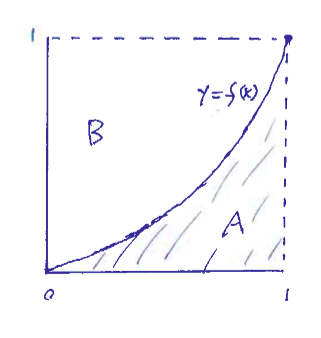
\includegraphics[width=\columnwidth]{idk.png}
	\end{figure}
	$B = $ Arealet av rektangelet $ - A$.
	\\
	Arealet er 1.
	B er derfor 
	\[1 - \frac{1}{\ln 2} - \frac{1}{2\ln^2 2}\]'
	\section{Tilfeldige oppgaver}
	\begin{gather*}
		\lim_{x\to\infty} x\left( \sqrt{\frac{1}{x} + 1} -1 \right)\\
		=\lim_{x\to\infty} \frac{\sqrt{\frac{1}{x} + 1} - 1}{\frac{1}{x}}\\
		=\lim_{x\to\infty} \frac{\left(\sqrt{\frac{1}{x} + 1} - 1\right)\left(\sqrt{\frac{1}{x} + 1} + 1\right)}{\frac{1}{x}\left(\sqrt{\frac{1}{x} + 1} + 1\right)}\\
		=\lim_{x\to\infty} \frac{\frac{1}{x} + 1 - 1}{\frac{1}{x}\left(\sqrt{\frac{1}{x} + 1} + 1\right)}\\
		=\lim_{x\to\infty} \frac{1}{\sqrt{\frac{1}{x} + 1} + 1}\\
		=\frac{1}{\sqrt{0 + 1} + 1}=\doubleunderline{\frac{1}{2}}
	\end{gather*}
	\rule{\columnwidth}{0.5pt}
	$x_0$ er et vilkårlig punkt. Vi skal ha
	\begin{gather*}
		|f(x) - f(x_0)| < \epsilon\\
		\Leftrightarrow |Ax+B - (Ax_0 + B)|<\epsilon|\\
		\Leftrightarrow |Ax - Ax_0|<\epsilon\\
		\Leftrightarrow |A(x-x_0)| < \epsilon
		\Leftrightarrow |A|\cdot|x-x_0| < \epsilon\\
		\Leftrightarrow |x-x_0|<\frac{\epsilon}{|A|}
	\end{gather*}
	For hver $\epsilon>0$, velg $\delta = \frac{\epsilon}{|A|}$, så vil
	\begin{gather*}
		0 < | x - x_0 | < \delta \implies |x-x_0|<\frac{\epsilon}{|A|}\\
		\implies |f(x) - f(x_0)|<\epsilon
	\end{gather*}
	Dermed er f kontinuerlig i $x_0$
	\rule{\columnwidth}{0.5pt}
	\begin{figure}[H]
		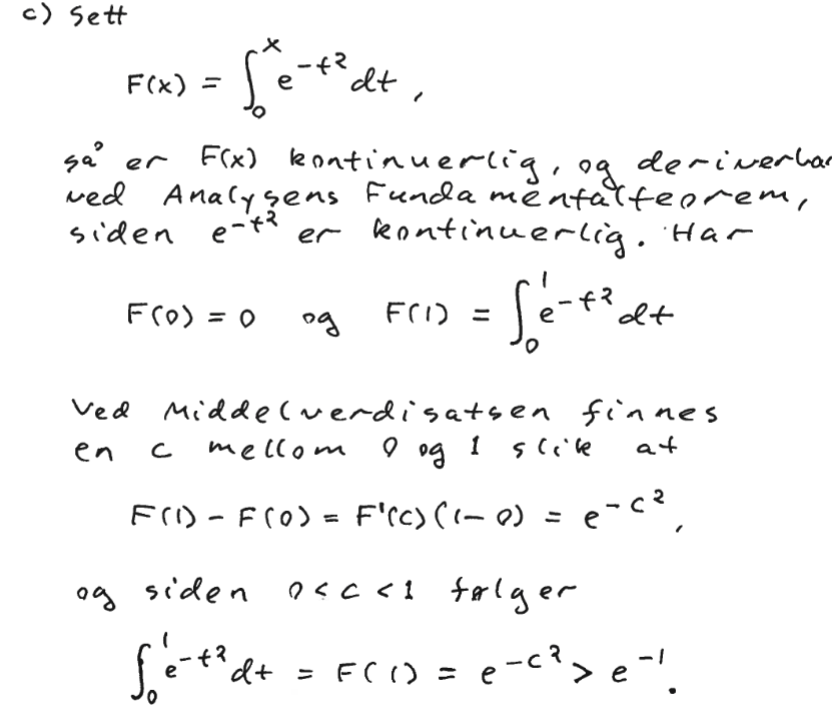
\includegraphics[width=\columnwidth]{idk2.png}
	\end{figure}
	
	\begin{center}
		
		\begin{tikzpicture}
			\duck[body=yellow!50!brown!40!white,
			crazyhair=gray!50!white,
			eyebrow,
			glasses=brown!70!black,
			book=\scalebox{0.28}{$e^{\pi i}=-1$},
			bookcolour=red!20!brown]
		\end{tikzpicture}
	\end{center}

	\cofeAm{0.5}{0.6}{180}{4.4cm}{12.03214cm}

	%\section{Kant}
	%\kant[10-30]

	%\section{Terje Vigen}
	%\input{terjevigen.txt}
\end{document}
